\chapter{Opis projektnog zadatka}

    \section{Motivacija i osnovna ideja}
    
        Broj napuštenih pasa u skloništima u Hrvatskoj, pa i ostalim europskim zemljama, svaki dan je sve veći i veći. Kao posljedica toga, psi u prosjeku provode sve više vremena u skloništu čekajući svog novog vlasnika. S druge strane, postoje brojni ljudi koji vole pse i žele im pomoći, ali nisu u mogućnosti udomiti psa, bilo zbog manjka prostora ili nedostatka vremena. \newline \\
        Jedan od najboljih načina na koji mogu pomoći, a da ne udome psa, je šetnjama. Tako se psima olakšava čekanje i smanjuje vrijeme provedeno u skloništu, te ga se ispunjava na koristan način – fizičkom aktivnošću i socijalizacijom.
        Ljudima se pruža prilika da uživaju u druženju sa psima, a možda da upoznaju i svog novog najboljeg prijatelja. \newline \\
        Kako je većina ljudi vrlo zaposlena ideja je stvoriti web aplikaciju koja bi na jednostavan i brz način spojila udruge za zaštitu životinja i zainteresirane građane-šetače pasa. Olakšavanjem postupka same prijave za šetnju i kreiranjem atraktivne aplikacije koja je lagana za korištenje, smatramo da bi se znatno povećao broj zainteresiranih građana. \newline \\
        Aplikacija je namijenjena dvjema skupinama krajnjih korisnika: građanima - potencijalnim šetačima pasa i udrugama za zaštitu životinja. \newline \\
        Prijavom u sustav udruge unose podatke o psima koje žele uključiti u aktivnost. Građani zatim mogu pregledati sve udruge i pse raspoložive za šetnju, te odabrati psa i rezervirati termin šetnje. Odabrani termin vidljiv je udruzi koja u dogovoreno vrijeme predaje psa šetaču. Aplikacija također vodi statistiku o svim provedenim šetnjama te ju, uz korisnikovu suglasnost, prikazuje javno u obliku rang liste najaktivnijih šetača.
        
    \section{Detaljan opis rješenja}
        \subsection{Općenito}
        
        Glavna namjena aplikacije je spajanje ljubitelja životinja s udrugama kojima je njihova pomoć, u vidu šetnji, potrebna. Aplikacija bi bila realizirana kao web aplikacija, uključujući i prilagodbu za prikaz na mobilnim uređajima. Bila bi dostupna na području države, te potencijalno korištena od strane većeg broja korisnika (pregledi zainteresiranih građana).
    
    \subsection{Vrste korisnika}
    
        Korisnik je svaka osoba, ne nužno registrirana, koja u bilo kojem trenutku pregledava ili koristi neki dio aplikacije. Razlikujemo dva tipa korisnika: šetače i udruge.
        \begin{packed_item}
            \item[1)] \textbf{Građani - šetači} \\
            Pod šetače spadaju svi korisnici koji aplikaciju upotrebljavaju s ciljem pronalaska psa za šetnju. Razlikujemo neregistrirane korisnike (javni posjetitelji) te registrirane korisnike.
            \begin{packed_item}
                        \item[a)] \textbf{Neregistrirani korisnici (javni posjetitelji)}\\
                        Jedan od glavnih ciljeva aplikacije je zainteresirati što veći broj ljudi za šetanje pasa. Stoga i neregistrirani korisnici imaju mogućnost pregleda profila svih udruga, profila njihovih pasa koji sudjeluju u programu, pregled statistika šetnje svih pasa unutar neke udruge te lokaciju same udruge. Statistika šetnji također nudi informacije o psima koji su manje šetani od ostalih te koji imaju veću potrebu za šetnjom. Korisniku se nudi i opcija prijave za šetanje pasa, a ako korisnik odabere tu opciju, korisnika se obavještava da kako bi napravio registraciju treba biti prijavljen u sustav.
            
                        \item[b)] \textbf{Registrirani korisnici} \\
                        Kako bi se korisnik registrirao za šetača, mora navesti:
                        \begin{packed_item}
                            \item[$\bullet$] ime
                            \item[$\bullet$] prezime
                            \item[$\bullet$] adresu e-pošte
                            \item[$\bullet$] željeno korisničko ime
                            \item[$\bullet$] lozinku
                        \end{packed_item}
                        
                        Nakon što korisnik obavi registraciju, ima opciju pregleda udruga i pasa raspoloživih za šetnju, isto kao i neregistrirani korisnik. Međutim, kao registriranom korisniku pružaju mu se i mogućnosti odabira psa za šetnju, odabir željenog termina te prijava za samu šetnju.  Nakon odabira termina šetnje, bilo javne ili grupne, korisniku se termin šetnje prikazuje u kalendaru, a svoj raspored može preuzeti i u PDF obliku.
                        Također, svi registrirani korisnici imaju opciju pregleda vlastitog profila, uključujući nadolazeće i prethodne šetnje, statistike, osobne podatke i slično. Mogu označiti vlastite statistike šetnji kao javne, u kojem slučaju se one mogu pojaviti na javnoj rang listi.
                        Imaju i opciju uređivanja svojih podataka, te brisanja računa na stranici.
            \end{packed_item}
            
            \item[2)] \textbf{Udruge} \\
                Kako bi se obavila registracija, udruga mora navesti:
                \begin{packed_item}
                    \item[$\bullet$] ime i prezime osobe koja predstavlja udrugu
                    \item[$\bullet$] adresu e-pošte
                    \item[$\bullet$] naziv udruge
                    \item[$\bullet$] OIB udruge
                    \item[$\bullet$] željeno korisničko ime
                    \item[$\bullet$] lozinku
                \end{packed_item}
                Nakon obavljene prijave, udruga može započeti sa stvaranjem profila za pse u svojem skrbništvu.
                \newline
                Za stvaranje profila jednog psa, udruga navodi sljedeće informacije:
                \begin{enumerate}
                    \item[$\bullet$] ime
                    \item[$\bullet$] slika (neobavezno)
                    \item[$\bullet$] opis psa
                    \item[$\bullet$] preferirani način šetnje
                        \begin{enumerate}
                            \item[$\bullet$] invidualna šetnja / šetnja s drugim psima
                        \end{enumerate}
                    \item[$\bullet$] vrsta
                \end{enumerate}
                Ti profili, zajedno sa osnovnim informacijama o udruzi te statistikama šetnji svih njenih pasa, javno su dostupni svim korisnicima web aplikacije. Udruga u bilo kojem trenutku može obrisati neki od profila pasa , u kojem slučaju se otkazuju i svi budući termini šetnji na koje je prijavljen. \newline \\
                Udruga također ima pristup svim rezervacijama za svoje pse, koje imaju opciju otkazati. \newline \\
                Udruga također ima opciju pregleda svojih podataka i uređivanja istih, kao i brisanja svog profila iz aplikacije. U tom slučaju se automatski brišu i profili svih pasa registriranih preko te udruge.
        \end{packed_item}
        \section{Opis funkcionalnosti aplikacije}
        \subsection{Pregled pasa / udruga}
        
            Ovo je jedna od glavnih funkcionalnost aplikacije. I registriranim i neregistriranim korisnicima omogućen je prikaz svih pasa koji sudjeluju u programu, te je omogućeno i filtriranje pasa prema lokaciji, udruzi, preferiranom načinu šetnje itd. Moguć je i pregled profila svih udruga, te pojedinih pasa o kojima neka udruga skrbi (a koji sudjeluju u programu) . \\
            
            \noindent Profil psa sadrži kratke informacije o psu, kao i njegovu sliku te termine u kalendaru i točno vrijeme kada je pas dostupan za šetnju. 
        
        \subsection{Rezervacija i potvrda termina šetnje}
        
            Nakon što korisnik pronađe psa kojeg želi šetati, sljedeći korak je rezervacija termina šetnje. Korisnik prvo pregledava termine u kalendaru kada je pas dostupan, te odabire termin koji mu odgovara. Ukoliko je korisnik odabrao psa koji voli grupne šetnje, tada korisnik u istom terminu može odabrati još jednog psa koji voli grupne šetnje, pod uvjetom da su iz iste udruge.

            
        \subsection{Pregled statistika}
        Postojio nekoliko vrsta statistike koje aplikacija vodi:
            \begin{enumerate}
                \item \textbf{Statistike šetača pasa}
                    \begin{enumerate}
                        \item[$\bullet$] uključuju broj šetnji, broj prošetanih pasa te ukupnu duljinu šetnji
                        \item[$\bullet$] po defaultu privatna statistika, korisnik ju sam može učiniti javnom, u kojem slučaju se prikazuje i na naslovnoj stranici, u sklopu liste najaktivnijih šetača
                    \end{enumerate}
                
                \item \textbf{Statistike udruge}
                    \begin{enumerate}
                        \item[$\bullet$] uključuje broj pasa u skrbi udruge te ukupan broj šetnji obavljen sa psima udruge
                        \item[$\bullet$] statistika javno dostupna svim korisnicima
                    \end{enumerate}
                    
                \item \textbf{Statistike admina}
                    \begin{enumerate}
                        \item[$\bullet$] ukupan broj aktivnih korisnika stranice
                        \item[$\bullet$] ukupan broj aktivnih udruga na stranici
                        \item[$\bullet$] ukupan broj pasa uključenih u program stranice
                    \end{enumerate}
            \end{enumerate}
        
    \section{Implementacijski detalji}
        Kako je jedan od glavnih ciljeva aplikacije privući što više korisnika u program, aplikacija mora podržavati istovremeni rad većeg broja korisnika. Za implementaciju backend dijela aplikacije odabran je programski jezik Java, uz pomoć frameworka Spring, dok je za frontend korišten React.\\
        
        \noindent Aplikacija se krajnim korisnicima prikazuje u obliku web-stranice, prilagođene za prikaz na mobilnim uređajima kao i na osobnim računalima.
        
    \section{Pregled konkurentskih rješenja i stanje tržišta}
    
        Najbliže konkurentske aplikacije su aplikacije za plaćeno šetanje pasa, poput BarkleyPets ( \url{https://barklypets.com/}), WagWalking(\url{https://wagwalking.com/}), DogHero (\url{https://play.google.com/store/apps/details?id=br.com.doghero.astro}) i slično. Iako ove aplikacije predstavljaju određenu konkurenciju, u smislu da ciljaju istu skupinu korisnika kao i naša aplikacija (ljude koje vole pse i žele provoditi vrijeme s nijima), naglasak naše aplikacije je na volontiranju, a ne na plaćenom šetanju, čime efektivno ipak korisnicima nudimo drugačiju vrstu usluge nego navedene aplikacije. \\
        
        \noindent Pod ostalu konkurenciju možemo svrstati forme za prijavu za volontiranje na stranicama raznih skloništa, poput \url{https://www.bluecross.org.uk/volunteer},  \url{https://helpingpaws.net/how-to-volunteer/}. Međutim, prijava preko formi na tim stranicama samo je prvi od mnogo koraka koje potencijalni volonter mora proći prije nego što mu se pruži prilika izvesti psa u šetnju. Naša aplikacija je i osmišljena da olakšava i ubrza postupak prijave za volontiranje, te eliminira potrebu za službenom prijavom poput navedenih. \\
        
        \noindent Također, bitno je naglasiti da navedene konkurentne aplikacije nisu bazirane na hrvatskom tržištu po ćemu se razlikuje naša aplikacija. Iz tog razloga, smatramo da naša aplikacija može pokriti dosad relativno neiskorišten dio tržišta, i uz pravi marketing, privući velik broj korisnika. \\
		
		 \noindent Dodatan korak koji smo odlučili napraviti da bismo dobili osjećaj o stvarnom interesu građana za ovakvu vrstu aplikacije, bilo je provođenje male verzije istrage tržišta. Koristeći alate koje nudi Google Forms, izradili smo javnu anketu i podijelili je među ljudima takozvanom \textit{chain message} metodom. Naime, poznanicima smo poslali anketu na ispunjavanje s prijateljskim prijedlogom da ju i oni podijele sa svojim poznanicima. Jasno je da takva statistika nije nepristrana, ali ipak daje dozu uvida u potražnju tržišta i dobra je polazna točka za ozbiljnija istraživanja u budućnosti. Na slici \ref{fig:anketa-interes} moguće je vidjeti rezultate odgovora na pitanje o interesu građana. 
        
        \begin{figure}[H]
		    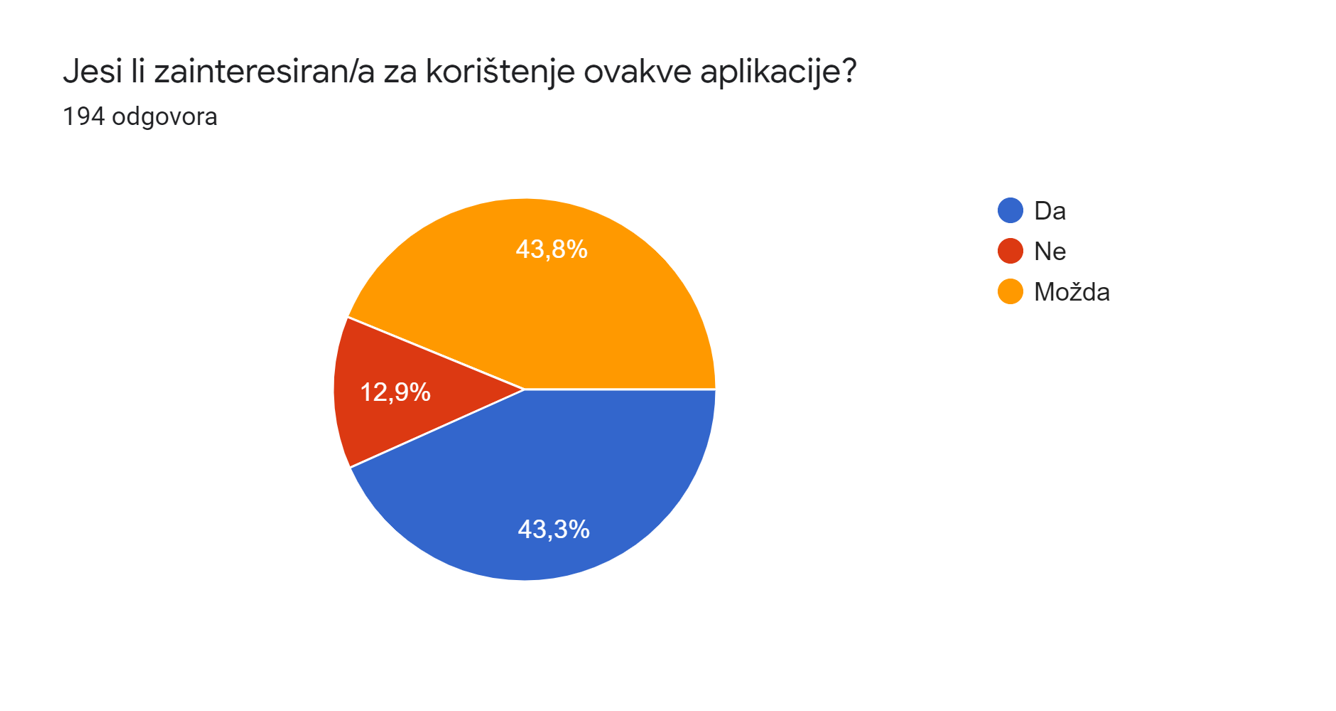
\includegraphics[scale=0.515]{slike/anketa-interes.PNG} 
		    \centering
		    \caption{Rezultat anketnog pitanja o interesu za aplikaciju}
		    \label{fig:anketa-interes}
	    \end{figure}
        
        \noindent Osim pitanja o interesu, naša je anketa služila i odabiru imena aplikacije. Vjerujemo da iza svake dobre aplikacije stoji pamtljivo ime koje ju dobro predstavlja. Uzevši prijedloge svih članova tima složili smo anketno pitanje o odabiru najboljeg i uključili ga u javnu anketu. Rezultat tog dijela ankete jasan je po naslovu dokumenta, a ostale prijedloge i detalje o rezultatu moguće je vidjeti na slici \ref{fig:anketa-ime}.
        
        
        \begin{figure}[H]
		    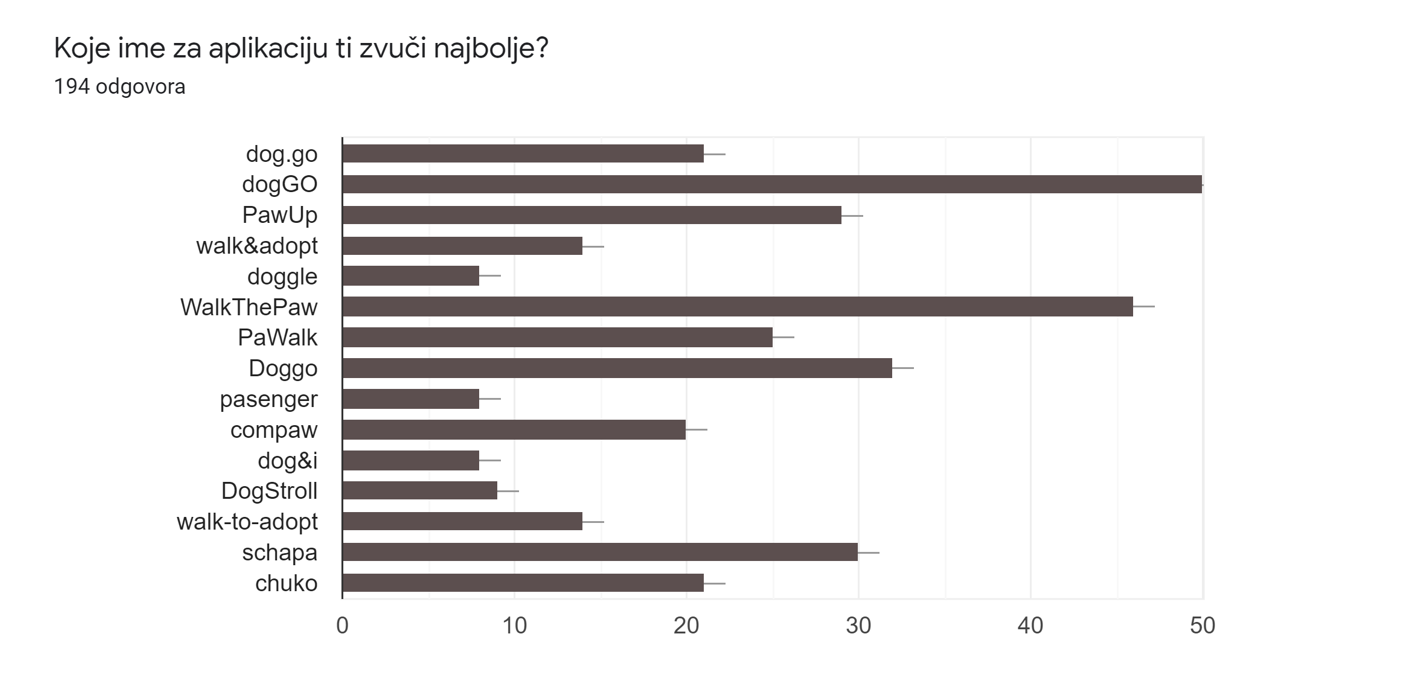
\includegraphics[scale=0.55]{slike/anketa-ime.PNG} 
		    \centering
		    \caption{Rezultat anketnog pitanja o imenu aplikacije}
		    \label{fig:anketa-ime}
	    \end{figure}
    